\chapter{Experiments and Results}\label{ch2:experiments-results}

\section{Experiments}\label{sec1:experiments} 

Here are some of the quantitative and qualitative evaluations of the variants of the recreated 2020 Single-View MPI model trained on different combinations of the Mannequin Challenge and RealEstate10K datasets. We use the pretrained weights of the 2020 MPI model as the benchmark and compare the abilities of all models at hand to generate novel views (more extensive training underway). We adopt some of the quantitative metrics from the 2020 MPI paper \cite{single_view_mpi} --- PSNR, SSMI \cite{wang_ssmi_psnr}, and LPIPS \cite{zhang2018perceptual} --- to give numeric values to the similarities between MPI-rendered video frames and the corresponding ground truth target frames the rendering process attempts to replicate. 

The following are the model variants used to compute the metrics stated above to help provide arguments for or against each of the hypotheses stated in section \ref{sec1:approach}: ---
\begin{itemize}
    \item The pretrained weights of the 2020 single-view MPI model trained exclusively on RealEstate10K data.
    \item The recreated 2020 model retrained exclusively on the Mannequin Challenge dataset with transfer learning using the pretrained weights of the original 2020 MPI model. In this transfer learning process, none of the layers of the pretrained weights were frozen and so could learn and evolve based on the Mannequin Challenge data they were newly exposed to.
    \item The recreated 2020 model retrained not just on the Mannequin Challenge dataset but also on the RealEstate10K dataset with similar transfer learning as in the previous variant. This variant was encouraged to be tried out by one of the authors of the 2020 MPI paper in our correspondences with him. \cite{single_view_mpi}
\end{itemize}

We sifted through the test set of the Mannequin Challenge dataset to hand pick a set of 333 videos that contained ORB-SLAM2 recognized sequences\footnote{the timestamp, camera intrinsics and extrinsics of all frames of each of which are listed in the corresponding .txt files in the dataset} which had video-chat-relevant features like the head and torso of people being focused on rather than having wide shots of entire bodies, the number of people in the frame being mostly limited to one or two as opposed to multiple people being featured, and the head pose of people being roughly or even very loosely aligned with the camera (there was hardly anybody that looked directly at the camera). We put them in the test-yes/ bin. We also curated test-maybe/ (311 videos) and test-no/ (25 videos) bins that consisted of the rest of the Mannequin Challenge test set with sequences either having no relevance to video chat (like there being hardly anyone in the frames) for test-no/ to those falling heavily in the gray areas between test-yes/ and test-no/ for test-maybe/. We even occasionally interspersed the test-yes/ and test-maybe/ bins with videos containing sequences that portrayed people facing diametrically opposite the camera just to really challenge the model variant being tested.

{\sloppy Of the various aspects of the code that we modelled from the textual descriptions and relevant code snippets procured from both the 2020 Single-View and 2018 Stereo MPI papers\footnote{Please find our code repository at \url{https://github.com/au001/view-synthesis.git}} like \verb`generator_test.py`, \verb`generator_train.py`, \verb`data_loader.py`, \verb`train.py`, and \verb`test.py`, the scripts relevant to the experiments in this section are test.py and generator\_test.py. For testing, the generator first aggregates all videos names from the directory input to it and for each of these, it picks reference\_image and target\_image to be either 5 or 10 frames apart. reference\_image is the frame that test.py uses to infer the MPI of the scene from and target\_image is supposedly a view of the same scene from a different angle. The possibility that, when the camera moves from one scene to another in the same video, reference\_image may depict a scene different from the one captured by target\_image is expected to be extremely rare as both datasets have been curated by a similar ORB-SLAM2 process like COLMAP. In such hypothetical cases, target\_image will be erroneously rendered by mpi.render() in rendered\_image. But since we take the mean of the computed metrics over hundreds of test.py processed reference\_image, target\_image pairs, we believe the final accuracies of a variant's mean metrics will not be off the tracks much and that they shall still be used to determine a variant’s performance satisfactorily. Each of the three metrics are calculated between target\_image and rendered\_image. We first test and compute metrics of frames 5 part and then we repeat the same test process for frames 10 apart just to show (as in the case of the 2020 MPI paper) that the longer the baseline between reference/source and target views, the less the accuracy will be of the rendered image. Moreover, we also calculate the metrics for all processed reference\_image, target\_image pairs, to catch the hypothetical anomalies of complete scene changes mentioned above.}  

Another jewel in our project was our attempt to parallelize training across multiple GPUs, which we believed would allow us to increase the batch size --- currently limited to 4 pairs of reference and target images along with their respective camera poses, intrinsics, and 3D points of the reference image --- and thereby let larger parts of our 70000+ training ready sequences with associated point clouds be used for learning by our recreated model. But, since TensorFlow's direct conversion procedure that would let standard single-GPU utilizing scripts become multi-GPU-faring is as yet still an evolving process requiring careful attention to resource allocation issues among the various replicas of the parallelizable aspects of the model --- like the dataset generator, the loss functions aggregator, etc. --- spread across GPUs, our training got undercut after a good start by the following error at training step 178: 

\begin{lstlisting}[breaklines]
    tensorflow.python.framework.errors_impl.ResourceExhaustedError: OOM when allocating tensor with shape[1,32,512,512,3] and type float on /job:localhost/replica:0/task:0/device:GPU:0 by allocator GPU_0_bfc [Op:StridedSlice] name: render/compose_back_to_front/strided_slice/
\end{lstlisting}

Nevertheless, we computed all three metrics for the second model variant retrained on Mannequin Challenge data but this time with \verb`tf.distribute.MirroredStrategy`, harnessing the power of multiple GPUs.

\section{Results}\label{sec:results} 

% The figures throughout the paper are
% best seen by zooming in to the electronic version of the paper.

% Figure: film reel of how a rerendered frame varies with change in head pose.

% 7.2) another main reason for would be due to our meticulous curating of the test set into multiple sub-test-sets characterized by the number of people in the shot, whether half or less than half of the person was captured in the frame, and how close the captured person(s) was to the camera.

The results for the experiments done on the baseline pretrained model and the variant retrained on only the video-chat-relevant Mannequin Challenge dataset are presented in this section. As of this writing \texttt{generator\_test.py} is only able to pick random pairs of reference and target frames from the 333 \texttt{test-yes/} videos. The results for sequential pair picking, which would avoid possible repetition of picked pairs and allow for an exhaustive coverage of the test set, will replace the results below in a subsequent manuscript of this thesis shortly alongside the results for the variant trained on both the Mannequin Challenge and RealEstate10K datasets and more visually appealing/insightful graphs. Moreover, the number of training iterations/steps will be much more than the current 10k steps which is projected to increase the accuracy even more. 

An LPIPS value of 0 indicates there is either a perfect match between the images being compared or the images being compared are one and the same. To the contrary, SSIM values of 1 indicate a perfect match. Both these metrics range from 0 to 1. PSNR values, measured in decibels (dB), don't generally have an upper limit but values 20 dB or higher are considered acceptable. In calibrating our implementations of these metrics, when we compared an image with itself, we found the mean LPIPS, SSIM and PSNR values over 300 images to be as follows:  

% \begin{appendices}

\newcolumntype{L}{>{\raggedleft\arraybackslash}m{3.5cm}}
\newcolumntype{M}{>{\raggedright\arraybackslash}m{2cm}}
\newcolumntype{N}{>{\centering\arraybackslash}m{1.5cm}}
\newcolumntype{O}{>{\centering\arraybackslash}m{3cm}}

\begin{table*}[t]
% \begin{sidewaystable*}[t]
    \centering
    \begin{tabular}{ML|NN|NN}
    \toprule
    
    & & \multicolumn{2}{O}{\textbf{LPIPS $\downarrow$} target\_image vs rendered\_image} & \multicolumn{2}{O}{\textbf{LPIPS $\downarrow$} reference\_image vs target\_image} \\
    
    \cmidrule(lr){3-4} \cmidrule(lr){5-6}
    
    \textbf{Model Variant} & \textbf{Dataset(s) (re)trained on / No. of Videos} & n = 5 & n = 10 & n = 5 & n = 10 \\
    \midrule
    
    Pretrained & RealEstate10K / $\sim$70k & 0.418 & 0.525 & 0.446 & 0.555 \\
    
    \cmidrule(lr){1-2} \cmidrule(lr){3-4} \cmidrule(lr){5-6}
    
    Recreated & Mannequin Challenge / 1841 & 0.319 & 0.433 & 0.446 & 0.555 \\
    
    \cmidrule(lr){1-2} \cmidrule(lr){3-4} \cmidrule(lr){5-6}
    
    Recreated  & Mannequin Challenge + RealEstate10K & -- & -- & -- & -- \\
    
    \cmidrule(lr){1-2} \cmidrule(lr){3-4} \cmidrule(lr){5-6}
    
    Recreated multi-GPU & Mannequin Challenge & 0.418 & 0.525 & 0.446 & 0.555 \\
    
    \bottomrule
    \end{tabular}
    \caption{LPIPS Mean Values}
    \label{tab:lpips}
    {\small n refers to the distance between the reference and target frames picked by the generator. Retraining promises marked improvement over original pretrained model.}
\end{table*}
% \end{sidewaystable*}

\begin{table*}[t]
% \begin{sidewaystable*}[t]
    \centering
    \begin{tabular}{ML|NN|NN}
    \toprule
    
    & & \multicolumn{2}{O}{\textbf{SSIM $\uparrow$} target\_image vs rendered\_image} & \multicolumn{2}{O}{\textbf{SSIM $\uparrow$} reference\_image vs target\_image} \\
    
    \cmidrule(lr){3-4} \cmidrule(lr){5-6}
    
    \textbf{Model Variant} & \textbf{Dataset(s) (re)trained on / No. of Videos} & n = 5 & n = 10 & n = 5 & n = 10 \\
    \midrule
    
    Pretrained & RealEstate10K / $\sim$70k & 0.549 & 0.492 & 0.418 & 0.370 \\
    
    \cmidrule(lr){1-2} \cmidrule(lr){3-4} \cmidrule(lr){5-6}
    
    Recreated & Mannequin Challenge / 1841 & 0.560 & 0.494 & 0.418 & 0.370 \\
    
    \cmidrule(lr){1-2} \cmidrule(lr){3-4} \cmidrule(lr){5-6}
    
    Recreated  & Mannequin Challenge + RealEstate10K & -- & -- & -- & -- \\
    
    \cmidrule(lr){1-2} \cmidrule(lr){3-4} \cmidrule(lr){5-6}
    
    Recreated multi-GPU & Mannequin Challenge & 0.549 & 0.492 & 0.418 & 0.555 \\
    
    \bottomrule
    \end{tabular}
    \caption{SSIM Mean Values}
    \label{tab:ssim}
    {\small n refers to the distance between the reference and target frames picked by the generator. Retraining promises marked improvement over original pretrained model.}
\end{table*}
% \end{sidewaystable*}

\begin{table*}[t]
% \begin{sidewaystable*}[t]
    \centering
    \begin{tabular}{ML|NN|NN}
    \toprule
    
    & & \multicolumn{2}{O}{\textbf{PSNR $\uparrow$} target\_image vs rendered\_image} & \multicolumn{2}{O}{\textbf{PSNR $\uparrow$} reference\_image vs target\_image} \\
    
    \cmidrule(lr){3-4} \cmidrule(lr){5-6}
    
    \textbf{Model Variant} & \textbf{Dataset(s) (re)trained on / No. of Videos} & n = 5 & n = 10 & n = 5 & n = 10 \\
    \midrule
    
    Pretrained & RealEstate10K / $\sim$70k & 16.105 & 14.088 & 13.185 & 11.589 \\
    
    \cmidrule(lr){1-2} \cmidrule(lr){3-4} \cmidrule(lr){5-6}
    
    Recreated & Mannequin Challenge / 1841 & 16.729 & 14.664 & 13.185 & 11.589 \\
    
    \cmidrule(lr){1-2} \cmidrule(lr){3-4} \cmidrule(lr){5-6}
    
    Recreated  & Mannequin Challenge + RealEstate10K & -- & -- & -- & -- \\
    
    \cmidrule(lr){1-2} \cmidrule(lr){3-4} \cmidrule(lr){5-6}
    
    Recreated multi-GPU & Mannequin Challenge & 16.105 & 14.088 & 13.185 & 11.589 \\
    
    \bottomrule
    \end{tabular}
    \caption{PSNR Mean Values}
    \label{tab:psnr}
    {\small n refers to the distance between the reference and target frames picked by the generator. Retraining promises marked improvement over original pretrained model.}
\end{table*}
% \end{sidewaystable*}

% % \end{appendices}

These metrics mean value tables produced via the random reference, target pair experiments so far validate hypothesis A of this thesis by showing that transfer learning with completely unfrozen layers seems to be helping the Single-View MPI pick up from where it left off by specializing and improve upon its performance in accurately predicting close up shots of people in video-chat-relevant frames. 

A further testimony to this improvement can be obtained by inspecting the performance of even the prematurely halted multi-GPU variant. It performs at par with the original pretrained model which indicates that the pretrained model has begun to continue where it left off and specialize in processing video-chat-like frames. It would have run properly if not for the resource errors mentioned in the previous section that could point to underlying issues like possible unchecked growth of TensorFlow graphs per pipeline replica or something else. This seems to be the case even though the replicas seem to be getting properly allocated inputs and their respective outputs also seem to be getting well gelled together in the end.

The authors of Single-view MPI paper used the following pointers like the handling of occluded content, the production unpleasant artifacts at the edges of foreground objects, and so on to qualitatively compare the discrepancies in the results generated by each variant model. In addition to visually checking for these, we, like the authors also found that visually checking the disparity maps is also useful in verifying the quality of the MPI produced.   

\begin{figure}[!h]
\begin{tabular}{cccc}
\subfloat[reference]{\includegraphics[width = 1.3in]{figures/pretrained-5-apt/000000_image_reference.png}} &
\subfloat[target]{\includegraphics[width = 1.3in]{figures/pretrained-5-apt/000000_image_target.png}} &
\subfloat[disparity]{\includegraphics[width = 1.3in]{figures/pretrained-5-apt/000000_image_disparity.png}} &
\subfloat[rendered]{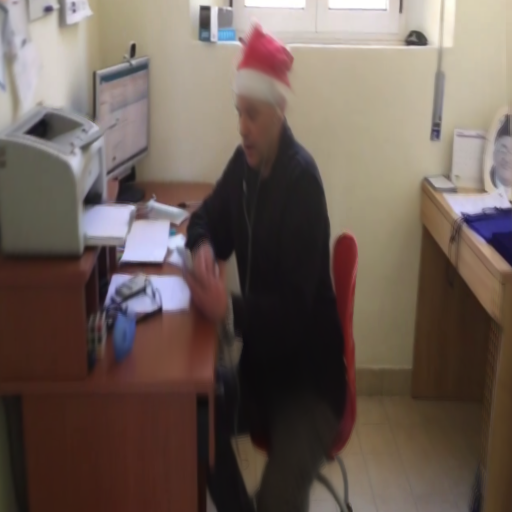
\includegraphics[width = 1.3in]{figures/pretrained-5-apt/000000_image_render.png}}\\
\subfloat[reference]{\includegraphics[width = 1.3in]{figures/mann-1841-5-apt/000000_image_reference.png}} &
\subfloat[target]{\includegraphics[width = 1.3in]{figures/mann-1841-5-apt/000000_image_target.png}} &
\subfloat[disparity]{\includegraphics[width = 1.3in]{figures/mann-1841-5-apt/000000_image_disparity.png}} &
\subfloat[rendered]{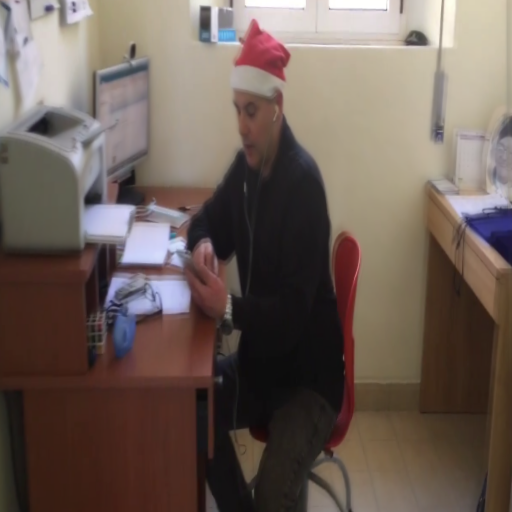
\includegraphics[width = 1.3in]{figures/mann-1841-5-apt/000000_image_render.png}}\\
\subfloat[reference]{\includegraphics[width = 1.3in]{figures/pretrained-10-apt/000000_image_reference.png}} &
\subfloat[target]{\includegraphics[width = 1.3in]{figures/pretrained-10-apt/000000_image_target.png}} &
\subfloat[disparity]{\includegraphics[width = 1.3in]{figures/pretrained-10-apt/000000_image_disparity.png}} &
\subfloat[rendered]{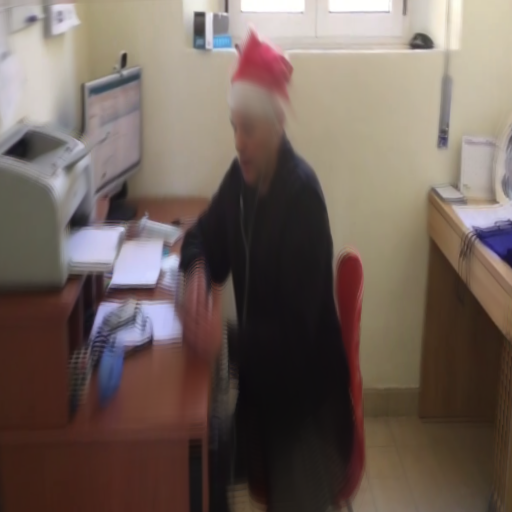
\includegraphics[width = 1.3in]{figures/pretrained-10-apt/000000_image_render.png}}\\
\subfloat[reference]{\includegraphics[width = 1.3in]{figures/mann-1841-10-apt/000000_image_reference.png}} &
\subfloat[target]{\includegraphics[width = 1.3in]{figures/mann-1841-10-apt/000000_image_target.png}} &
\subfloat[disparity]{\includegraphics[width = 1.3in]{figures/mann-1841-10-apt/000000_image_disparity.png}} &
\subfloat[rendered]{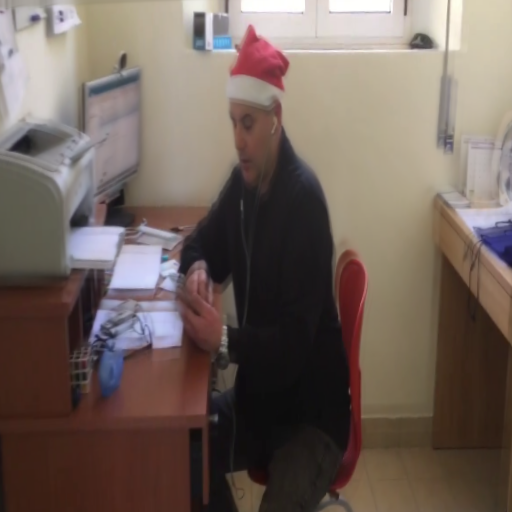
\includegraphics[width = 1.3in]{figures/mann-1841-10-apt/000000_image_render.png}}
\end{tabular}
\caption{Model Variants' Output Visualizations}
    {\small First Row: Pretrained Model -- tested 5 frames apart; Second Row: Retrained Model -- trained on 1841 Mannequin Challenge videos -- tested 5 frames apart; Third Row: Pretrained Model -- tested 10 frames apart; Fourth Row: Retrained Model -- trained on 1841 Mannequin Challenge videos -- tested 10 frames apart}
\end{figure}